\documentclass[letterpaper,12pt]{article} % use larger type; default would be 10pt
\usepackage{amsbsy, geometry, graphicx}
\geometry{letterpaper}

\title{Extended Kalman Filter for SOC\\Stanford Solar Car}
\author{Bryant Tan}

\begin{document}
\maketitle

\tableofcontents

\newpage

\section{Introduction}

\subsection{Terms}

\begin{tabular}{ l l }
SOC & State of Charge \\
EKF & Extended Kalman Filter
\end{tabular}

\subsection{State of Charge}

The Stanford Solar Car is powered from a battery pack that is, over the course of the race, charged from the solar array and drained by the motor. In order to maximise the car's range, it is imperative to make an accurate estimate of the pack's state of charge.\\

It is possible to obtain measurements of the pack's voltage. Discharge curves (voltage against SOC) can be obtained from datasheets. These curves, however, are very flat over a large interval, and any data obtained from interpolating SOC from voltage will have large error bars.\\

The car also has an on-board coulomb counter which, for every 100ms interval, obtains a value for the average current over that interval from a microchip and sums these values over a longer time period. This measurement, however, is subject to drift.\\

A Kalman filter can be used to reconcile these measurements to produce an accurate estimate of SOC.

\newpage

\section{Theory}

\subsection{Extended Kalman Filter}

Each iteration of the EKF is a two-step process.\\

At the predict step, an estimate of the new state $ \hat{\boldsymbol{x}}_{k-1|k} $ and covariance $ \boldsymbol{P}_{k|k-1} $ is made given the previous state estimate $ \hat{\boldsymbol{x}}_{k-1|k-1} $ and a control variable $  \boldsymbol{u}_{k-1} $ (which represents external factors) based on an iteration function $ f(\boldsymbol{x}, \boldsymbol{u}) $ and a covariance $ \boldsymbol{Q}_{k-1} $ representing the confidence of the prediction.\\

At the update step, an improved estimate of the new state $ \hat{\boldsymbol{x}}_{k|k} $ and covariance $ \boldsymbol{P}_{k|k} $ is made given an instantaneous observation $ \boldsymbol{z}_{k} $, its covariance $ \boldsymbol{R}_{k} $ and the observation function $ h(\boldsymbol{x}) $ that maps state to an observable value.\\

Predict
\begin{equation}
\hat{\boldsymbol{x}}_{k|k-1} = f(\hat{\boldsymbol{x}}_{k-1|k-1}, \boldsymbol{u}_{k-1})
\end{equation}
\begin{equation}
\boldsymbol{P}_{k|k-1} =  {\boldsymbol{F}_{k-1}} \boldsymbol{P}_{k-1|k-1}{\boldsymbol{F}_{k-1}^\top} + \boldsymbol{Q}_{k-1}
\end{equation}

Update
\begin{equation}
\tilde{\boldsymbol{y}}_{k} = \boldsymbol{z}_{k} - h(\hat{\boldsymbol{x}}_{k|k-1})
\end{equation}
\begin{equation}
\boldsymbol{S}_{k} = \boldsymbol{H}_{k}\boldsymbol{P}_{k|k-1}\boldsymbol{H}_{k}^\top + \boldsymbol{R}_{k}
\end{equation}
\begin{equation}
\boldsymbol{K}_{k} = \boldsymbol{P}_{k|k-1}\boldsymbol{H}_{k}^\top\boldsymbol{S}_{k}^{-1}
\end{equation}

\begin{equation}
\hat{\boldsymbol{x}}_{k|k} = \hat{\boldsymbol{x}}_{k|k-1} + \boldsymbol{K}_{k}\tilde{\boldsymbol{y}}_{k}
\end{equation}
\begin{equation}
\boldsymbol{P}_{k|k} = (I - \boldsymbol{K}_{k} \boldsymbol{H}_{k}) \boldsymbol{P}_{k|k-1}
\end{equation}\\

I'll be using a one-dimensional implementation of an EKF in which the single hidden variable is SOC ($x$).

\newpage

\subsection{The Model}

The prediction function $ f(x, \Delta x) $ is given by

\begin{equation}
\hat{x}_{k|k-1} = f(\hat{x}_{k-1}, \Delta x) = \hat{x}_{k-1} + \Delta x
\end{equation}

where $ \Delta x $ can be obtained from the coulomb counter. The covariance $ Q_k $ can be calculated based on the magnitude of $ \Delta x $ and supplied as a parameter to the iteration step. \\

Of course,
\begin{equation}
\frac{\partial}{\partial x} f(x, \Delta x) = 1
\end{equation}
\begin{equation}
\boldsymbol{F}_{k-1} = \left . \frac{\partial f}{\partial \boldsymbol{x} } \right \vert _{\hat{\boldsymbol{x}}_{k-1|k-1},\boldsymbol{u}_{k-1}} = [1]
\end{equation}


The observation function $ h_{\theta}(x) $ and its associated covariance function $ R_{\theta}(x) $ can be obtained from data taken from multiple discharge curves. Both parametrised by $ \theta $, temperature. At every iteration of the EKF, they will be re-generated based on the current pack temperature by interpolating data from discharge curves.\\

This gives the following update and predict steps:\\

Predict
\begin{equation}
\hat{x}_{k|k-1} = \hat{x}_{k-1} + \Delta x
\end{equation}
\begin{equation}
P_{k|k-1} =  P_{k-1|k-1} + Q_{k-1}
\end{equation}

Update
\begin{equation}
H_k = \left. \frac{\partial}{\partial x}h_\theta(x) \right \vert _{\hat{x}_{k|k-1}}
\end{equation}
\begin{equation}
\tilde{y}_k = z_k - h_\theta(\hat{x}_{k|k-1})
\end{equation}
\begin{equation}
S_{k} = {H_k}^2 P_{k|k-1} + R_k
\end{equation}
\begin{equation}
K_k = P_{k|k-1} H_k {S_k}^{-1}
\end{equation}

\begin{equation}
\hat{x}_{k|k} = \hat{x}_{k|k-1} + K_k\tilde{y}_k
\end{equation}
\begin{equation}
P_{k|k} = (1 - K_k H_k) P_{k|k-1}
\end{equation}

\section{Observables}

There are two important processes that need to be characterised: the coulomb counter and the mapping from voltage measurements to SOC (i.e. the functions $f$ and $h$).

\subsection{Coulomb Counter}

The coulomb counter can be hacked to be a joule counter and operate in the following way: over the course of 100ms, the counter integrates current to produce a highly accurate measure of the amount of charge that has passed over that period. At the end of each 100ms block it reports this value as well as the mean voltage across the battery pack over that period. This should give a measurement of the amount of energy the pack has supplied.\\

The measurement we want is $ \int V \, dq \equiv \int V  \frac {dq} {dt} \, dt \equiv \int I V \, dt $. The measurement we get from the coulomb counter is $ \langle V \rangle \int I \, dt \equiv  \frac { 1 }{ \Delta t } \int V \, dt \int I \, dt $, which is not strictly equivalent. However, since the two quantities become equal when V(t) is constant over the interval and this is likely to be approximately the case for most intervals given the brevity of 100ms, this approximation is probably sufficiently accurate.

\subsection{Voltage}

As the pack discharges from a full charge, a plot of voltage against energy used looks like this (here voltage is on the y-axis and time in seconds is on the x-axis; a constant power was drawn from the battery using a BK programmable load):\\

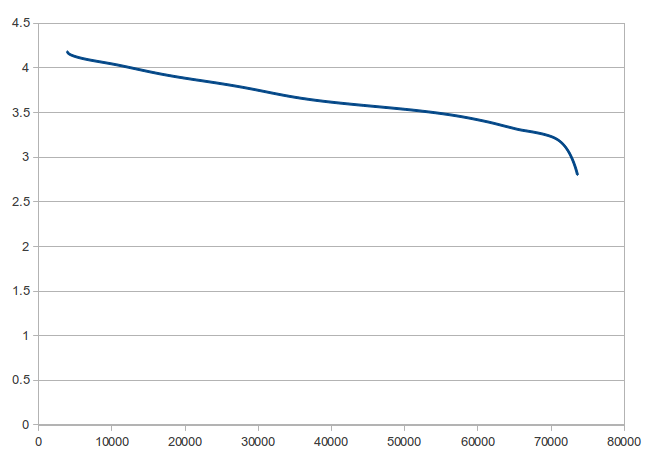
\includegraphics[width=140mm]{discharge_curve.png}\\

This discharge curve does not, however, fully characterise $h(x)$, as the function is temperature-dependent. Further, the pack is affected by voltage lift and sag when current is flowing in and out of the pack respectively. Since real cells can be modelled as ideal cells in series with a resistor, the amount of lift and sag is proportional to the current entering and leaving the cell.

\section{Test Plan}

I have access to a large number of single battery cells. The entire pack consists of 35 batteries wired in series, each of which consists of 13 cells in parallel. Running tests on a single battery should give enough information to model the entire pack.\\

\subsection{Coulomb Counter}

The function $ f(x, \Delta x) = x + \Delta x $ is very simple, and all that needs to be determined is the covariance; namely the degree to which $ \Delta x $ measured by the counter agrees with actual $ \Delta x $. This can be easily determined by running several discharge curves using a programmable load set to constant power.

\subsection{Voltage}

\end{document}
